\subsection{Earlier Tests: When Spatial Filtering Helps}
\begin{figure*}[!t]
\centering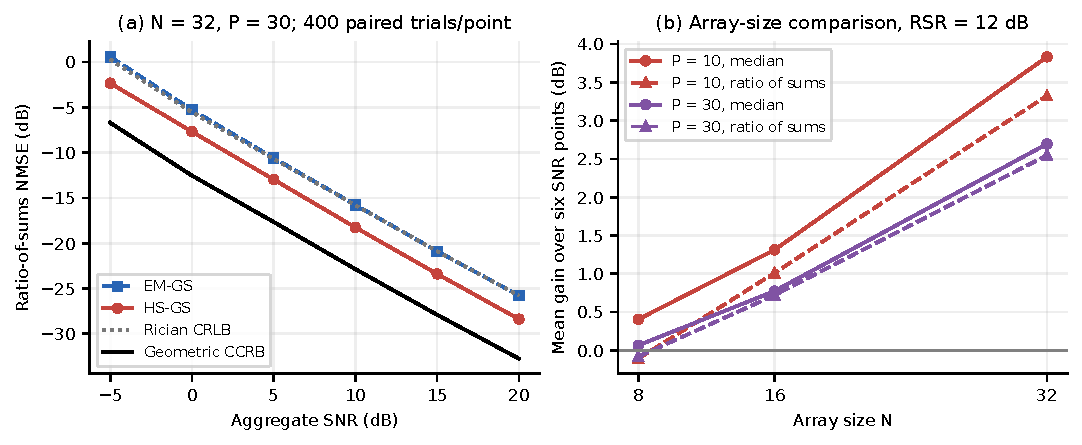
\includegraphics[width=\textwidth]{classical_array.pdf}
\caption{Earlier classical study. Left: channel error and information references for 32 antennas and 30 pilots. Right: gain from HS-amplitude filtering as array size grows. HS-GS uses four filtering sweeps. Solid lines average paired-median gains over six SNRs; dashed lines combine squared errors within each setting before averaging gains. These are separate tests from Table~\ref{tab:reliability-main}.}
\label{fig:classical}
\end{figure*}
The earlier array study uses 400 shared channel draws per setting, three users, 10 or 30 pilots and RSR 12~dB. With 32 antennas and 30 pilots, hard Hankel filtering improves the paired-median error over EM-GS by 2.54--2.97~dB across six SNRs (Fig.~\ref{fig:classical}). Averaging the pilot counts and SNRs gives gains of 0.236, 1.044 and 3.264~dB for 8, 16 and 32 antennas. Larger arrays provide more samples of the same spatial paths. The information curves describe local unbiased-estimation limits, not a guaranteed gain for the filters.

To describe how strongly the channel is concentrated in a few spatial components, define the effective rank~\cite{royvetterli2007}
\begin{equation}
 r_{\rm eff}=\exp(-\textstyle\sum_i p_i\log p_i),\qquad \rho=r_{\rm eff}/q.
\end{equation}
A low value means a few singular values carry most of the channel. Here $\rho$ is calculated from the true channel for analysis; the receiver cannot use it.
\begin{figure}[!t]
\centering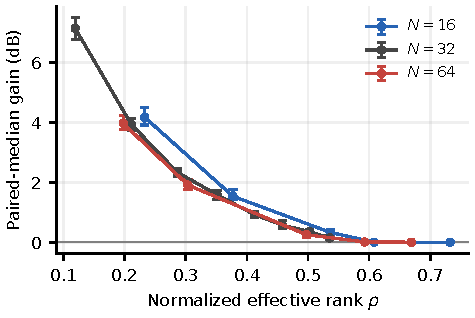
\includegraphics[width=\columnwidth]{effective_rank.pdf}
\caption{Earlier structure test. Hard-filter gain falls as more spatial components become important. The horizontal axis uses the true channel and cannot serve as an online switching rule. Bars show pointwise paired-bootstrap intervals. The arrays use 20 pilots, RSR 10~dB and the same random-SNR distribution.}
\label{fig:rank}
\end{figure}
Figure~\ref{fig:rank} shows that hard filtering generally helps less as $\rho$ rises. At $N=32$ and $\rho=0.536$, the median gain is only 0.141~dB. At $N=16$, $L=14$ and $\rho=0.732$, forcing rank seven loses 0.154~dB. A value near one-half marks a small gain in this test, not a general threshold. At 32 antennas, 14 paths and SNR 0~dB, even selected-rank filtering is worse than EM-GS in 47.75\% of draws. Smooth classical filtering improves on four hard sweeps by 0.914--1.413~dB in the tested 0~dB cases. Thus learning is not required to improve hard truncation, and more filtering is not always better.
